\chapter{fMRI model specification \label{Chap:fmri_spec}}

Statistical analysis of fMRI data uses a mass-univariate approach based on General Linear Models (GLMs). It comprises the following steps (1) specification of the GLM design matrix, fMRI data files and filtering (2) estimation of GLM parameters using classical or Bayesian approaches and (3) interrogation of results using contrast vectors to produce Statistical Parametric Maps (SPMs) or Posterior Probability Maps (PPMs).

The design matrix defines the experimental design and the nature of hypothesis testing to be implemented.  The design matrix has one row for each scan and one column for each effect or explanatory variable. (eg. regressor or stimulus function). You can build design matrices with separable session-specific partitions.  Each partition may be the same (in which case it is only necessary to specify it once) or different.

Responses can be either event- or epoch related, the only distinction is the duration of the underlying input or stimulus function. Mathematically they are both modeled by convolving a series of delta (stick) or box functions (u), indicating the onset of an event or epoch with a set of basis functions.  These basis functions model the hemodynamic convolution, applied by the brain, to the inputs.  This convolution can be first-order or a generalized convolution modeled to second order (if you specify the Volterra option). The same inputs are used by the Hemodynamic model or Dynamic Causal Models which model the convolution explicitly in terms of hidden state variables.

Event-related designs may be stochastic or deterministic.  Stochastic designs involve one of a number of trial-types occurring with a specified probability at successive intervals in time.  These probabilities can be fixed (stationary designs) or time-dependent (modulated or non-stationary designs).  The most efficient designs obtain when the probabilities of every trial type are equal. A critical issue in stochastic designs is whether to include null events. If you wish to estimate the evoked response to a specific event type (as opposed to differential responses) then a null event must be included (even if it is not modeled explicitly).

\begin{figure}
\begin{center}
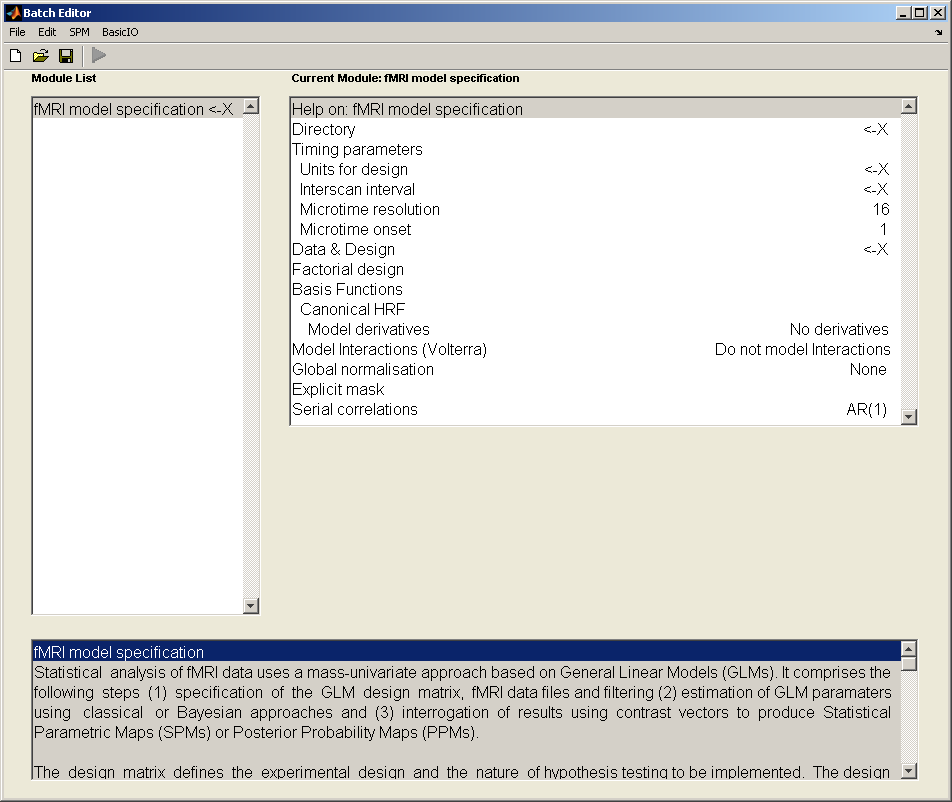
\includegraphics[width=100mm]{fmri_spec/fmri_model}
\end{center}
\caption{\em After starting SPM in fMRI mode and pressing the ``Specify 1st-level'' button, the SPM batch editor window should appear as above. The options for ``fMRI model specification'' can be examined by clicking on them. A single click will bring up some help text in the lower subwindow (not shown in the above graphic). Options highlighted with a ``$<$-X'' are mandatory and must be filled in by the user. Each of the options shown above is described in this chapter. \label{spec}}
\end{figure}

In SPM, analysis of data from multiple subjects typically proceeds in two stages using models at two ``levels''. The ``first level'' models are used to implement a within-subject analysis. Typically there will be as many first level models as there are subjects. Analysis proceeds as described using the ``Specify first level'' and ``Estimate'' options. The results of these analyses can then be presented as ``case studies''. More often, however, one wishes to make inferences about the population from which the subjects were drawn. This is an example of a ``Random-Effects (RFX) analysis'' (or, more properly, a mixed-effects analysis). In SPM, RFX analysis is implemented using the ``summary-statistic'' approach where contrast images from each subject are used as summary measures of subject responses. These are then entered as data into a ``second level'' model.

Figure~\ref{spec} shows how the SPM graphics window appears during fMRI model specification.

\section{Timing parameters}

Specify various timing parameters needed to construct the design matrix. This includes the units of the design specification and the interscan interval.

Also, with long TRs you may want to shift the regressors so that they are aligned to a particular slice.  This is effected by changing the microtime resolution and onset.

\subsection{Units for design}

The onsets of events or blocks can be specified in either scans or seconds.

\subsection{Interscan interval}

Interscan interval, TR, (specified in seconds).  This is the time between acquiring a plane of one volume and the same plane in the next volume.  It is assumed to be constant throughout.

\subsection{Microtime resolution}

In Echo-Planar Imaging (EPI), data is acquired a plane at a time. To acquire a whole volume of data takes at least a second or two.

It is possible, however, that experimental events may occur between scan (volume) acquisition times. This can be specified when building your design matrix either by (i) specifying your design in scans and using non-integer values  or (ii) specifying your design in seconds at a resolution greater than the TR.

SPM takes these timing specifications and builds its regressors using a `microtime' time-scale. The microtime resolution, t, is the number of time-bins per scan.

Do not change this parameter unless you have a long TR and wish to shift regressors so that they are aligned to a particular slice.

\subsection{Microtime onset}

The microtime onset, t0, is the first time-bin at which the regressors are resampled to coincide with data acquisition.  If t0 = 1 then the regressors will be appropriate for the first slice.  If you want to temporally realign the regressors so that they match responses in the middle slice then make t0 = t/2 (assuming there is a negligible gap between volume acquisitions).

Do not change the default setting unless you have a long TR. 

A typical use of the t and t0 parameters is to set them to correspond to the results of any slice timing correction you have made eg. if you have 24 slices and have made slice 12 the reference slice you would set t=24, t0=12. 

\section{Data \& Design}

The design matrix defines the experimental design and the nature of hypothesis testing to be implemented.  The design matrix has one row for each scan and one column for each effect or explanatory variable. (e.g. regressor or stimulus function).  Figure~\ref{design} shows an example of a design matrix.

\begin{figure}
\begin{center}
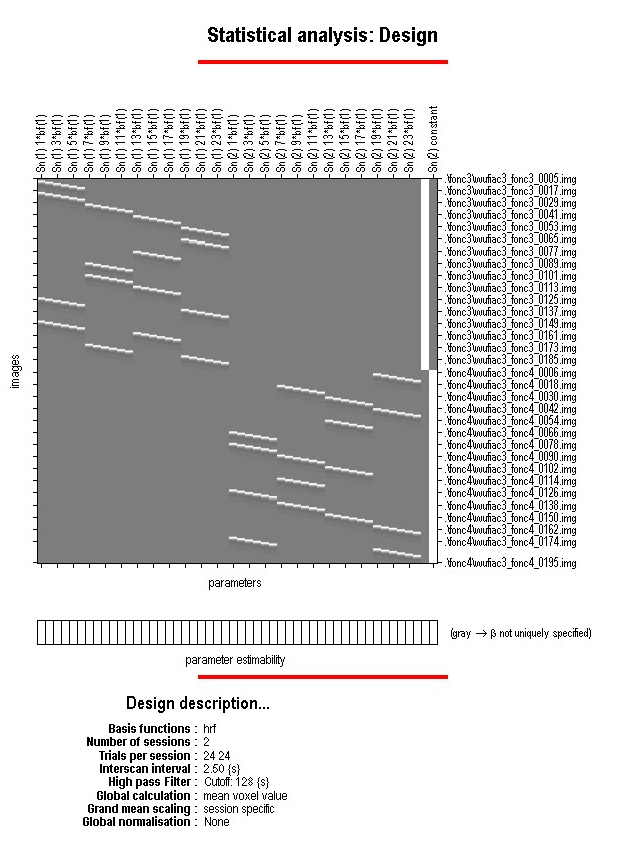
\includegraphics[width=100mm]{fmri_spec/design}
\end{center}
\caption{\em Design matrix for fMRI data from two sessions. There are 24 experimental conditions for each session. The last two columns model the average activity in each session, giving a total of 50 regressors. There are 191 fMRI scans for each session. The overall design matrix therefore has 382 rows and 50 columns. \label{design}}
\end{figure}

You can build design matrices with separable session-specific partitions.  Each partition may be the same (in which case it is only necessary to specify it once) or different.  Responses can be either event- or epoch related, where the latter model involves prolonged and possibly time-varying responses to state-related changes in experimental conditions.  Event-related response are modelled in terms of responses to instantaneous events.  Mathematically they are both modelled by convolving a series of delta (stick) or box-car functions, encoding the input or stimulus function. with a set of hemodynamic basis functions.

\subsection{Subject/Session}

The design matrix for fMRI data consists of one or more separable, session-specific partitions.  These partitions are usually either one per subject, or one per fMRI scanning session for that subject.

\subsubsection{Scans}

Select the fMRI scans for this session.  They must all have the same image dimensions, orientation, voxel size etc. This is implemented using SPM's file selector.

\subsubsection{Conditions}

You are allowed to combine both event- and epoch-related responses in the same model and/or regressor. Any number of condition (event or epoch) types can be specified.  Epoch and event-related responses are modeled in exactly the same way by specifying their onsets [in terms of onset times] and their durations.  Events are specified with a duration of 0.  If you enter a single number for the durations it will be assumed that all trials conform to this duration.For factorial designs, one can later associate these experimental conditions with the appropriate levels of experimental factors. 

\paragraph{Condition}

An array of input functions is constructed, specifying occurrence events or epochs (or both). These are convolved with a basis set at a later stage to give regressors that enter into the design matrix. Interactions of evoked responses with some parameter (time or a specified variate) enter at this stage as additional columns in the design matrix with each trial multiplied by the [expansion of the] trial-specific parameter. The 0th order expansion is simply the main effect in the first column.

\subparagraph{Name}

Condition Name

\subparagraph{Onsets}

Specify a vector of onset times for this condition type. This can be entered using the keyboard eg. typing in ``100 300'' and then hitting return or ``100;300'' or ``[100,300]'' or ``[100,300]''.

More usually, however, this specification takes place using variables that have been created before and loaded into matlab. For example, an \verb!my_onsets! cell array\footnote{Cell arrays are usually used in preference to matrices as different event types can then have different numbers of events.} might exist in a file you created earlier called \verb!my_design.mat!. You would then type \verb!load my_design! at the matlab command prompt before pressing the `Specify 1st-level' button. 

You could then specify the onsets for condition 2 by typing in eg. \verb!my_onsets{2}! instead of entering the numbers via the keyboard.


\subparagraph{Durations}

Specify the event durations. Epoch and event-related responses are modeled in exactly the same way but by specifying their different durations.  Events are specified with a duration of 0.  If you enter a single number for the durations it will be assumed that all trials conform to this duration. If you have multiple different durations, then the number must match the number of onset times.

\subparagraph{Time Modulation}

This option allows for the characterisation of nonstationary responses. Specifically, you can model either linear or nonlinear time effects. For example, 1st order modulation would model the stick functions and a linear change of the stick function heights over time. Higher order modulation will introduce further columns that contain the stick functions scaled by time squared, time cubed etc.

\subparagraph{Parametric Modulations}

The stick function itself can be modulated by some parametric variate (this can be time or some trial-specific variate like reaction time) modeling the interaction between the trial and the variate. The events can be modulated by zero or more parameters.

See \cite{parametric_pet,parametric_fmri} for further details of parametric modulations.

\subsubsection{Multiple conditions}

If you have multiple conditions then entering the details a condition at a time is very inefficient. This option can be used to load all the required information in one go. 

You will need to create a \verb!*.mat! file containing the relevant information. This \verb!*.mat! file must include the following cell arrays: names, onsets and durations eg. \verb!names{2}='SSent-DSpeak'!, \verb!onsets{2}=[3 5 19 222]!, \verb!durations{2}=[0 0 0 0]! contain the required details of the second condition. These cell arrays may be made available by your stimulus delivery program eg. COGENT. The duration vectors can contain a single entry if the durations are identical for all events. 

You then need to use SPM's file selector to select this \verb!*.mat! file.

\subsubsection{Regressors}

Regressors are additional columns included in the design matrix, which may model effects that would not be convolved with the haemodynamic response.  One such example would be the estimated movement parameters, which may confound the data.

\paragraph{Regressor}

\subparagraph{Name}

Enter name of regressor eg. First movement parameter

\subparagraph{Value}

Enter the values that the regressor takes. This could also be, for example, the name of a variable in MATLAB's work space that you have previously loaded in from a file. This might be a subjects movement parameters or reaction times.

\subsubsection{Multiple regressors}

If you have mutliple regressors eg. realignment parameters, then entering the details a regressor at a time is very inefficient. This option can be used to load all the required information in one go. 

You will first need to create a \verb!*.mat! file containing a matrix R. Each column of R will contain a different regressor. When SPM creates the design matrix the regressors will be named R1, R2, R3, ..etc.

You then need to use SPM's file selector to select this \verb!*.mat! file.

\subsubsection{High-pass filter}

The default high-pass filter cutoff is 128 seconds. Slow signal drifts with a period longer than this will be removed. Use ``Explore design'' to ensure this cut-off is not removing too much experimental variance. This is described later in section~\ref{explore}. High-pass filtering is implemented using a residual forming matrix (i.e. it is not a convolution) and is simply a way to remove confounds without estimating their parameters explicitly.  The constant term is also incorporated into this filter matrix.

\section{Factorial design}

If you have a factorial design then SPM can automatically generate the contrasts necessary to test for the main effects and interactions.

This includes the F-contrasts necessary to test for these effects at the within-subject level (first level) and the simple contrasts necessary to generate the contrast images for a between-subject (second-level) analysis.

To use this option, create as many factors as you need and provide a name and number of levels for each.  SPM assumes that the condition numbers of the first factor change slowest, the second factor next slowest etc. It is best to write down the contingency table for your design to ensure this condition is met. This table relates the levels of each factor to the conditions.

For example, if you have 2-by-3 design  your contingency table has two rows and three columns where the the first factor spans the rows, and the second factor the columns. The numbers of the conditions are 1,2,3 for the first row and 4,5,6 for the second.

See \cite{rnah_anova} for more information on SPM and factorial designs.

\subsection{Factor}

Add a new factor to your experimental design.

\subsubsection{Name}

Name of factor, eg. 'Repetition' 

\subsubsection{Levels}

Enter number of levels for this factor, eg. 2

\section{Basis Functions}

SPM uses basis functions to model the hemodynamic response. This could be a single basis function or a set of functions. The most common choice is the `Canonical HRF' with or without time and dispersion derivatives. 

\subsection{Canonical HRF}

Canonical Hemodynamic Response Function (HRF). This is the default option. Contrasts of these effects have a physical interpretation and represent a parsimonious way of characterising event-related responses. This option is also useful if you wish to look separately at activations and deactivations. This is implemented using a t-contrast with a +1 or -1 entry over the canonical regressor. 

\subsubsection{Model derivatives}

Model HRF Derivatives. The canonical HRF combined with time and dispersion derivatives comprise an `informed' basis set, as the shape of the canonical response conforms to the hemodynamic response that is commonly observed. The incorporation of the derivative terms allow for variations in subject-to-subject and voxel-to-voxel responses. The time derivative allows the peak response to vary by plus or minus a second and the dispersion derivative allows the width of the response to vary by a similar amount. 

A positive estimate of the time-derivative regression coefficient implies that the peak hemodynamic response occurs earlier than usual ie. than would be expected using just the canonical regressor. A positive estimate for the dispersion derivative implies a less dispersed response than usual.

The informed basis set requires an SPM{F} for inference. T-contrasts over just the canonical are perfectly valid but assume constant delay/dispersion. The informed basis set compares favourably with eg. FIR bases on many data sets \cite{rnah_basis}.

\subsection{Other basis sets}

The other basis sets supported by SPM are

\begin{enumerate}
\item{Fourier Set}
\item{Fourier Set (Hanning)}
\item{Gamma Functions}
\item{Finite Impulse Response (FIR)}
\end{enumerate}

For each of these options you must also specify the {\bf window length} which is the length in seconds of the post-stimulus time window that the basis functions span. You must also specify the {\bf order}, that is, how many basis functions to use.

Usually, an informed basis set should be sufficient for most data sets. If this does not provide a good fit to the data it may be worthwhile re-considering how the neuronal events are modelled ie. is the timing correct ? should events be split into subsets ? 

Alternatively, the gamma basis functions are an interesting choice as a particular linear combination of them is actually used to specify the canonical HRF. The FIR approach is of interest as it is equivalent to the method of `selective averaging'. See \cite{rnah_conv} for further details. 

\section{Model Interactions (Volterra)}

Generalized convolution of inputs, $U$, with basis set, $bf$.

For first order expansions the causes are simply convolved (e.g. stick functions) in $U$ by the basis functions in $bf$ to create a design matrix $X$.  For second order expansions new entries appear that correspond to the interaction among the original causes. The basis functions for these effects are two dimensional and are used to assemble the second order kernel. 

Interactions or response modulations can enter at two levels.  Firstly the stick function itself can be modulated by some parametric variate. This can be time or some trial-specific variate like reaction time modeling the interaction between the trial and the variate. Secondly interactions among the trials themselves can be modeled using a Volterra series formulation that accommodates interactions over time (and therefore within and between trial types). 

This last option is useful for accommodating nonlinearities in the hemodynamic response. For example, if two events occur within a second or so of each other then the hemodynamic response to the pair may be less than the sum of the responses to each event when occuring in isolation. This type of `sub-linear' response can be modelled using Volterra kernels. See \cite{balloon} for further details.

\section{Directory}

Select a directory where the SPM.mat file containing the specified design matrix will be written. If this directory already contains an SPM.mat file then SPM will warn you of this before overwriting it, when the specification job is run.

\section{Global normalisation}

SPM can normalise fMRI data in one of two ways. These are selected using the options `None' (the default) and `Scaling'.

Both methods are based on first estimating the average within-brain fMRI signal, $g_{ns}$, where $n$ denotes scan and $s$ denotes session. If you select `Scaling', SPM will multiply each fMRI value in scan $n$ and session $s$ by $100/g_{ns}$.

If you select ``None'' then SPM computes the grand mean value, $g_s=\frac{\sum_{n=1}^N g_{ns}}{N}$ where N is the number of scans in that session. This is the fMRI signal averaged over all voxels within the brain and all time points within session $s$. SPM then implements ``Session-specific grand mean scaling'' by multiplying each fMRI data point in session $s$ by $100/g_s$.

See \cite{ja_global} for further discussion of this issue.

\section{Explicit mask}

Specify an image for explicitly masking the analysis. A sensible option here is to use a segmentation of structural images to specify a within-brain mask. If you select that image as an explicit mask then only those voxels in the brain will be analysed. This both speeds the estimation and restricts SPMs/PPMs to within-brain voxels. Alternatively, if such structural images are unavailable or no masking is required, then leave this field empty.

\section{Serial correlations}

Serial correlations in fMRI time series due to aliased biorhythms and unmodelled neuronal activity can be accounted for using an autoregressive AR(1) model during Classical (ReML) parameter estimation.  

This estimate assumes the same correlation structure for each voxel, within each session.  ReML estimates are then used to correct for non-sphericity during inference by adjusting the statistics and degrees of freedom appropriately. The discrepancy between estimated and actual correlations are greatest at low frequencies.  Therefore specification of the high-pass filter is particularly important.

Serial correlation can be ignored if you choose the ``none'' option. Note that the above options only apply if you later specify that your model will be estimated using the Classical (ReML) approach. If you choose Bayesian estimation these options will be ignored. For Bayesian estimation, the choice of noise model (AR model order) is made under the estimation options. See \cite{peb1,vb_fmri_ar} for further discussion of these issues.

\section{Reviewing your design \label{explore}}

After you have completed the SPM ``job'' file for specifying your fMRI design, and have run it, you will then be able to review your design by pressing the ``Review'' button in SPM's button window (the top-left window). This is particularly useful, for example, for checking that your experimental variance has not been removed by high-pass filtering, as shown in Figure~\ref{rev4}.

\begin{figure}
\begin{center}
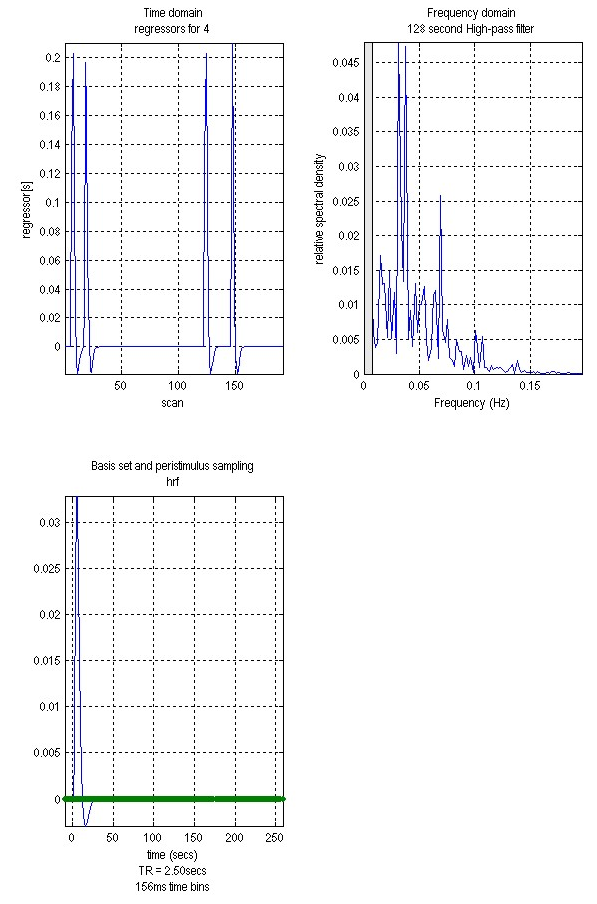
\includegraphics[width=100mm]{fmri_spec/reg4}
\end{center}
\caption{\em After pressing ``Review'', selecting the pull-down `Design' menu, Explore-$>$Session, and selecting the regressor you wish to look at, you should get a plot similar to the one above. The top row shows time and frequency domain plots of the time-series corresponding to this regressor. In this particular case we have four events. Each event or ``stick function'' has been convolved with the hemodynamic response function shown in the bottom panel. The frequency domain graph is useful for checking that experimental variance is not removed by high-pass filtering. The grayed out section of the frequency plot shows those frequencies which are removed. For this regressor we have plenty of remaining experimental variance (see the peak at about 0.04Hz). \label{rev4}}
\end{figure}
